\section{Simulation Results}
The simulation results are categorized into two components: the nominal (deterministic) environment and the stochastic environment.


In a nominal environment with no parameter deviation ($\delta_p = 0\%$), RL, MPC, and RL-MPC algorithms were simulated and trained using a deterministic prediction model($\hat{p}(k) = \mu_p$). This setup ensures that repeated simulations yield identical results. The nominal environment was crucial for developing the RL-MPC algorithm and evaluating the effectiveness of RL in providing useful terminal constraints and cost functions. Additionally, it served as the basis for generating the nominal trajectories for states and inputs.

In the stochastic environment, we test three levels of uncertainty: $\delta_p = 5\%$, $10\%$, and $20\%$. For these cases, MPC and RL-MPC continue to use a deterministic prediction model. However, three RL agents are trained, each specifically for one level of uncertainty. The stochastic environment is used to evaluate whether RL can impart its knowledge of the system's uncertainty to the EMPC, enabling the resulting RL-MPC algorithm to better handle the present uncertainty. Although the RL-MPC formulation relies on a deterministic prediction model, it leverages the RL agents’ knowledge of uncertainties. For each level of uncertainty, the RL-MPC’s initial guesses, terminal constraints, and terminal cost function are derived from the RL agent trained for that specific uncertainty level. Finally, prediction horizons of 1-6 hours were tested for the MPC and RL-MPC. Lastly, modification to the RL-MPC is made to ease the computational burden and tested against the original RL-MPC. For all simulations it was decided to have $\delta_T = 5\%$.

\subsubsection{Performance Metrics}
The performance metrics include the final cumulative reward achieved over the simulation period. This reward is the sum of stage costs, which encompasses \autoref{eq:optimisation-goal}, along with penalties for state and output violations. In other words, the sum of stage costs of \autoref{eq:reward_fn} or \autoref{eq:mpc_ocp}. Performance metrics for the nominal case will also include the computational time of each algorithm. For the stochastic setting, the performance metrics are detailed by including the mean final cumulative reward, averaged across 30 simulation runs, as well as the variance of the final cumulative reward.\\
To note, time series plots of the evolution of the system's states and inputs are not shown, since they are similar to those posted in \cite{morcegoReinforcementLearningModel2023, jansenOptimalControlLettuce2023, boersmaRobustSamplebasedModel2022}.

\subsection{Deterministic}
 \autoref{fig:rl-mpc-nominal} displays the performance and the computational time of the RL, MPC and the RL-MPC algorithms with various prediction horizons. 
\begin{figure}[h]
	\centering
	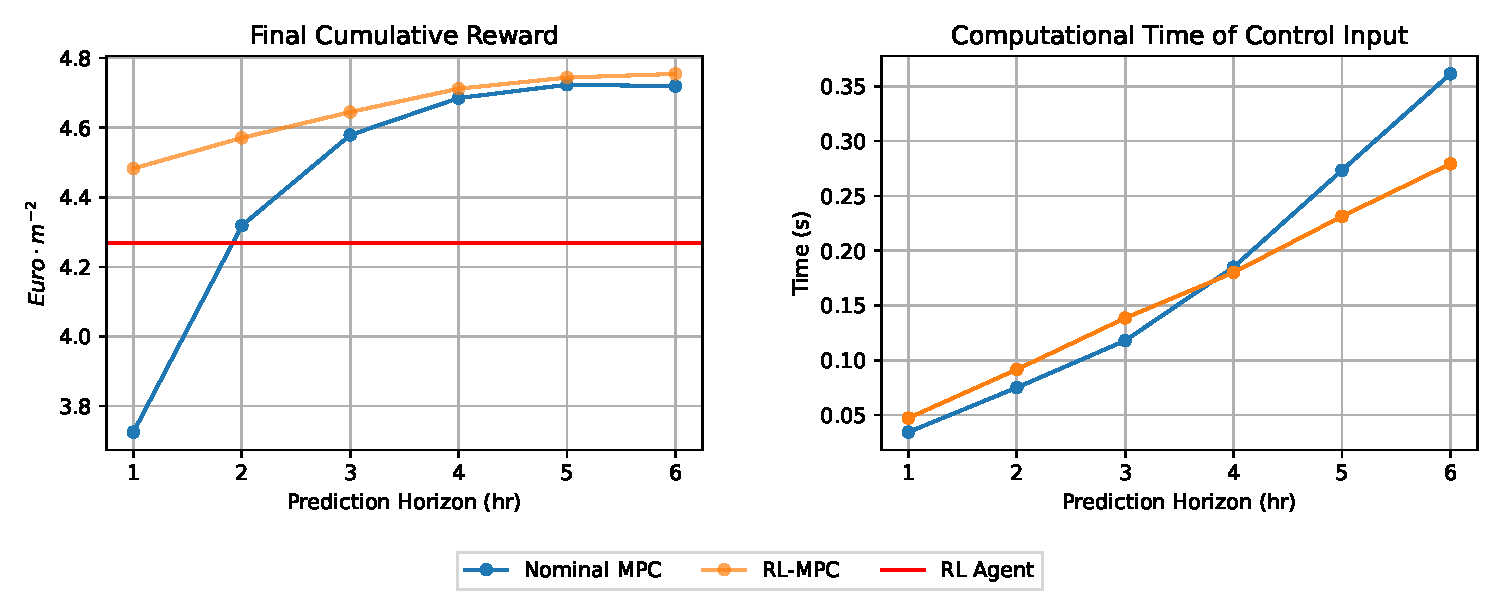
\includegraphics[width=\linewidth]{figures/rl_mpc_impl_final_research.pdf}
	\caption{Comparison of RL, MPC and RL-MPC on the nominal environment}
	\label{fig:rl-mpc-nominal}
\end{figure}
 It is clear that MPC is not myopic as previously thought. It noticeable outperforms the RL agent, with increased performance as prediction horizons increases, however; naturally, the computational time also increases. One could argue that it might not be necessary to introduce terminal constraints and a cost function from RL since performance of the EMPC is satisfactory. However, introducing these constraints and cost function boosts performance further across all prediction horizons, and significantly so at lower prediction horizons. Although the addition of a neural network as a cost function increases the computational time, it was found that the addition of the terminal constraints significantly lowers it to the point where the complete RL-MPC algorithm is faster the original MPC at higher prediction horizons. At lower prediction horizons, specifically 1 and 2 hours, the trade off between increased performance and increased computational costs is clearly in favour of increased performance. It is important to note that these terminal constraints and cost function are provided by an RL policy that performs considerably worse than MPC; however, they still visibly improve the RL-MPC performance. This demonstrates the importance of providing an EMPC with appropriate terminal constraints and cost functions to achieve superior performance.\\  
Lastly, one could argue that since the computational speeds are relatively fast compared to the control time interval (sub-second computational speeds versus a 30-minute interval), the prediction horizon can be increased until performance requirements are met. However, this model of the greenhouse system is relatively simple. More complex models may not offer the same flexibility in extending the prediction horizon.

\subsection{Stochastic}
Stochastic results are presented in \autoref{fig:rl-mpc-stochastic} and \autoref{fig:rl-mpc-stochastic-10}
\begin{figure}[h]
	\centering
	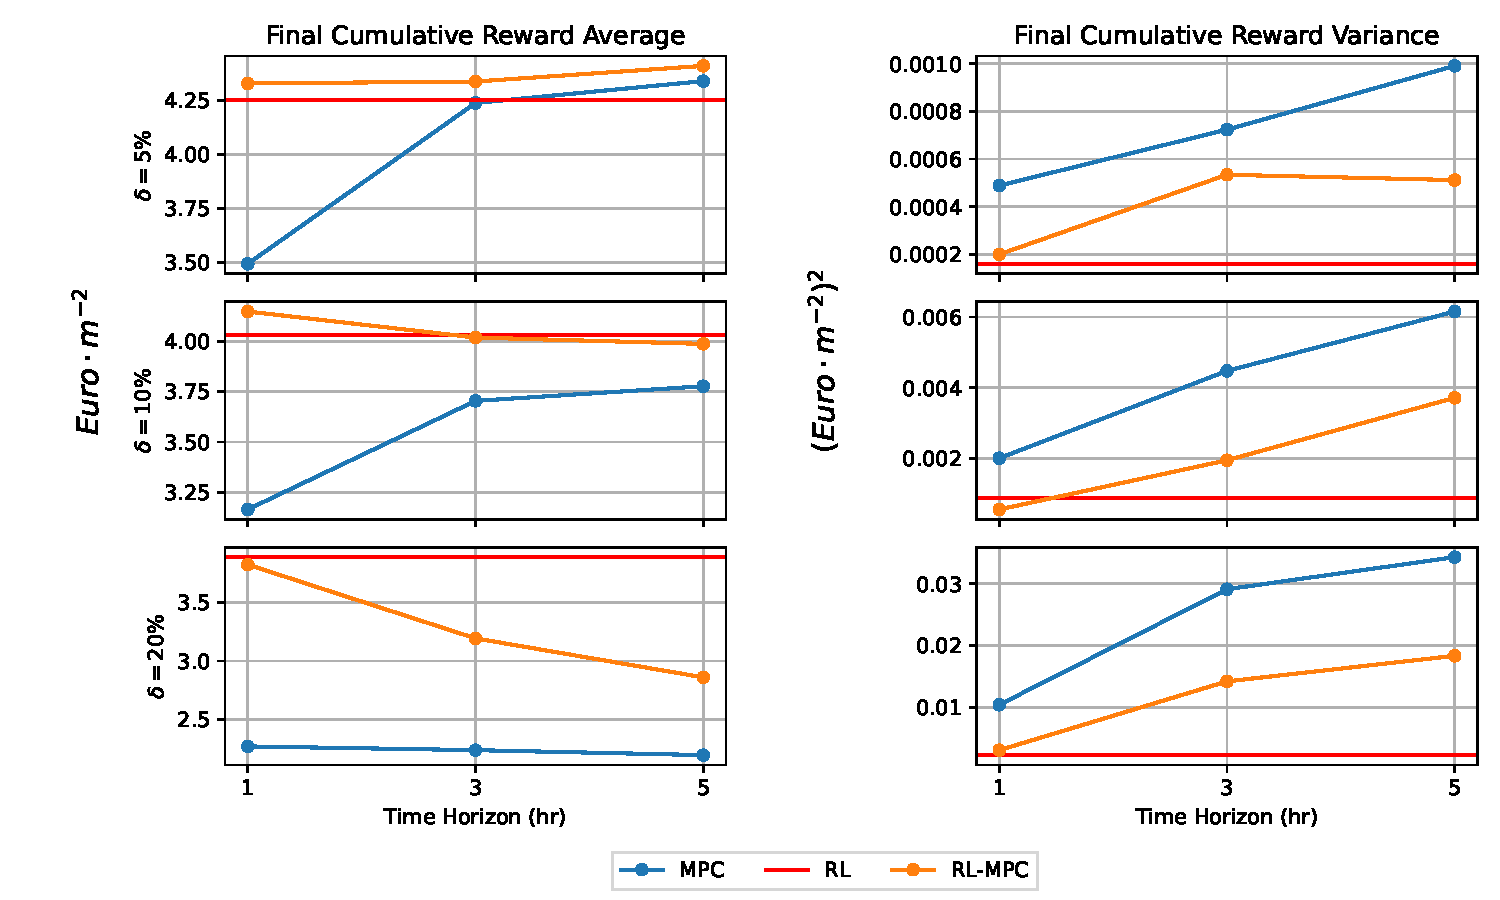
\includegraphics[width=\linewidth]{figures/stochastic_rl_vs_mpc_impl3.eps}
	\caption{Comparison of RL, MPC and RL-MPC across all prediction horizons}
	\label{fig:rl-mpc-stochastic}
\end{figure}
\autoref{fig:rl-mpc-stochastic} presents the findings of RL, MPC, and RL-MPC in a stochastic environment with varying levels of uncertainty across 1, 3, and 5-hour prediction horizons. It is evident that as uncertainty increases, RL outperforms MPC due to RL's ability to learn and manage uncertainty. Moreover, increasing the prediction horizon for MPC under higher uncertainty yields diminishing performance returns. The variance of RL is significantly lower than that of MPC, with the difference increasing as uncertainty rises.\\
In the case of RL-MPC, similar to the nominal scenario, at low uncertainties, RL-MPC outperforms both MPC and RL in terms of final mean cumulative reward. For all levels of uncertainty, RL-MPC noticeably outperforms MPC in both cumulative reward and variance across all prediction horizons. This demonstrates that the terminal constraints and cost function provided by RL impart knowledge of the uncertainty in the environment. Although RL still outperforms RL-MPC at higher levels of uncertainty, RL-MPC performs substantially better than the original EMPC.

Often, a conservative estimate of the uncertainty in the environment is used to develop a controller. Hence, \autoref{fig:rl-mpc-stochastic-10} includes the performance of an RL agent trained on data with $\delta_p = 10\%$, the RL-MPC algorithm that uses this agent, and the original MPC tested across three different uncertainty levels. The prediction horizon for the MPC and RL-MPC was fixed at 3 hours.

\begin{figure}[h]
	\centering
	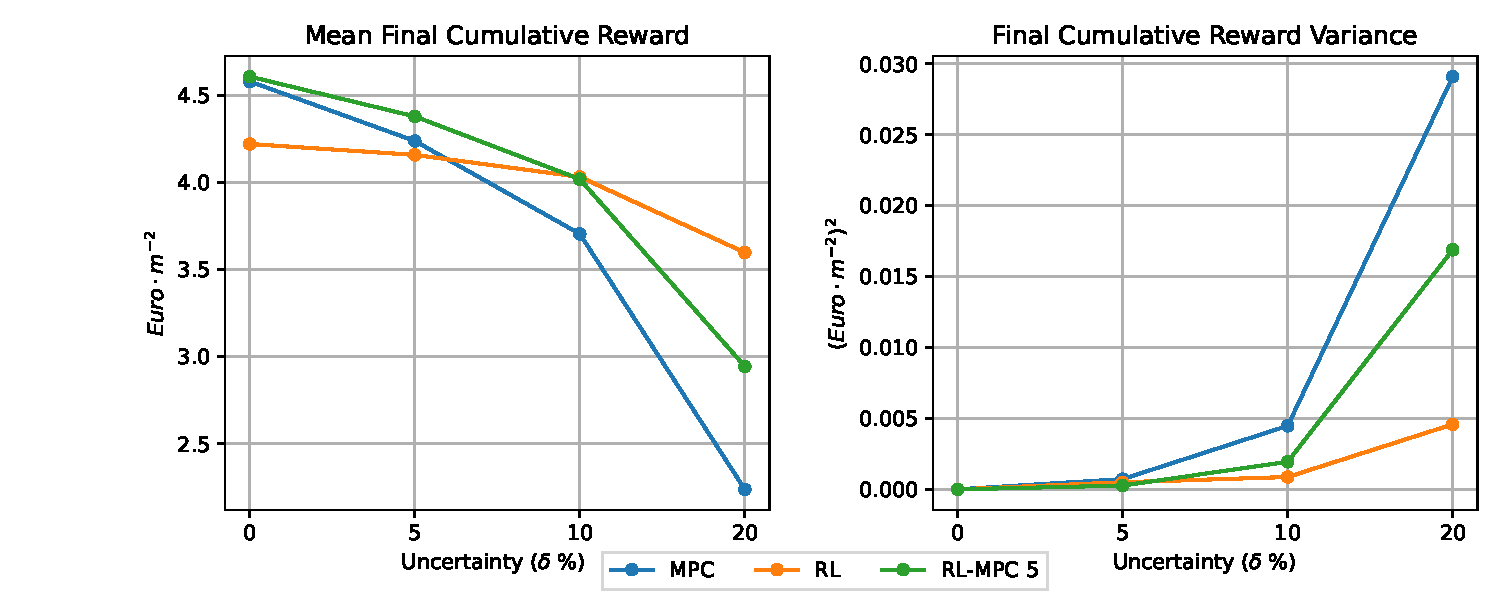
\includegraphics[width=\linewidth]{figures/stochastic_realife.eps}
	\caption{Comparison of RL, MPC and RL-MPC developed at $\delta_p = 10\%$}
	\label{fig:rl-mpc-stochastic-10}
\end{figure}

The superiority of the RL-MPC controller over both MPC and RL is illustrated in \autoref{fig:rl-mpc-stochastic-10}, particularly regarding mean final cumulative reward at low uncertainty levels. This trend persists until uncertainty reaches a threshold where MPC's performance noticeably declines, which negatively affects the RL-MPC's performance. Despite this, RL-MPC consistently outperforms MPC, showing a less severe performance drop as uncertainty increases. The RL agent remains the best performer under high uncertainty. \autoref{fig:rl-mpc-stochastic-10} suggests that equipping an EMPC with terminal constraints and a cost function generated by an RL agent trained on stochastic data enhances the EMPC's understanding and management of system uncertainty. Essentially, this approach makes the EMPC more robust against noise without sacrificing performance at lower uncertainty levels, and even enhances it.


\subsection{Speedup}
Although the original MPC and RL-MPC offer real-time computational speeds across all prediction horizons, RL-MPC may not be real-time for more complex systems due to the added computational burden from the neural network used as a cost function. Simplifying the neural network architecture and using approximations can help address this issue. While it was found that reducing the network size can improve computational speeds without performance loss, the focus here is on using Taylor approximations of the neural network around the terminal guess provided by RL. The results of this approach are shown in \autoref{fig:rl-mpc-speedup}.

\begin{figure}[h]
	\centering
	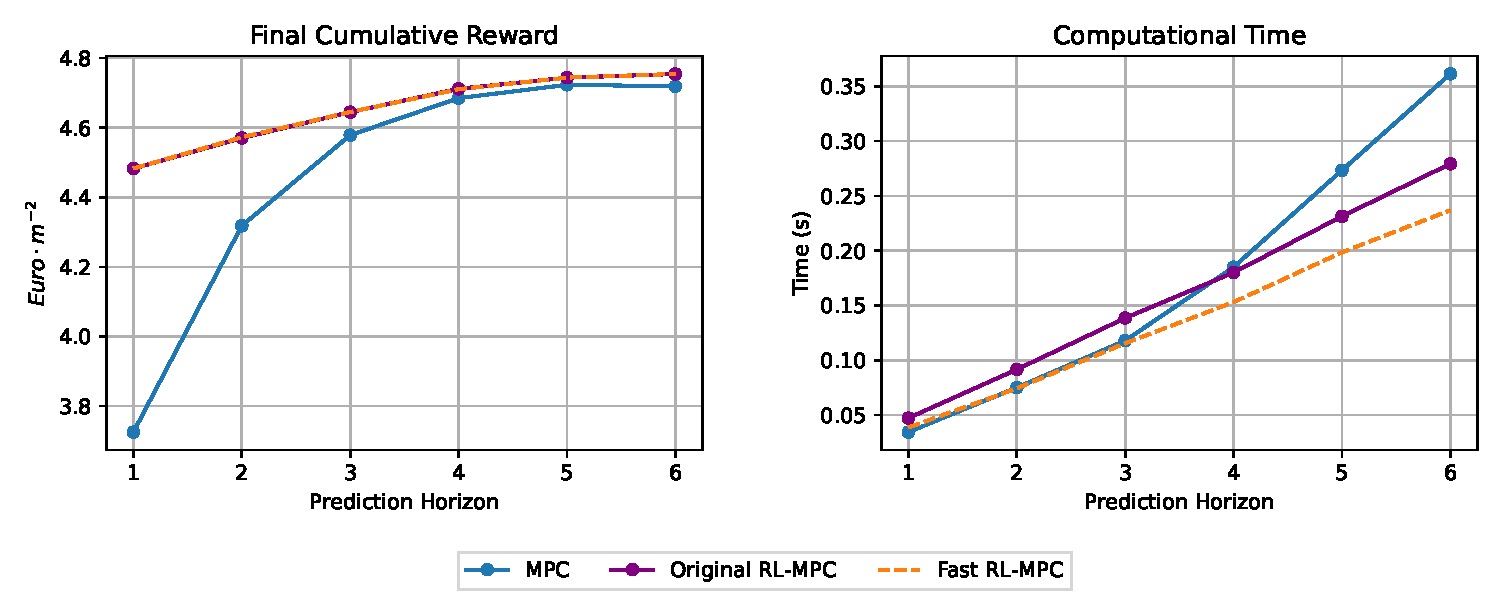
\includegraphics[width=\linewidth]{figures/final_speed_up.pdf}
	\caption{Fast RL-MPC}
	\label{fig:rl-mpc-speedup}
\end{figure}


It was found that a second-order Taylor approximation did not provide any advantage over a first-order approximation and hence not shown here. \autoref{fig:rl-mpc-speedup} illustrates that the first-order Taylor approximation results in a substantial increase in computational speeds without sacrificing performance, making the RL-MPC algorithm as fast as MPC at shorter prediction horizons. This approach is both simple and highly effective for making the RL-MPC algorithm faster.
